% Boss test of book/style.sty: every Writer-interface element. Not book content.
\documentclass[11pt,a4paper,oneside,openany]{book}
\usepackage{style}
\addbibresource{references.bib}
\graphicspath{{../../book/figures/}}
\begin{document}
\tableofcontents
\chapter{בדיקת סגנון}
\section{כותרת משנה}
טקסט רגיל עם \term{סינון שיתופי}{collaborative filtering} ומילה באנגלית \en{Spotify}, מספר 344 ואחוז 41\%.
ציטוט יחיד \cite{hu2008collaborative} וציטוט כפול \cite{koren2009matrix,resnick1994grouplens} ועם עמוד \cite[p.~3]{schedl2018current}.
\begin{scene}נועה עולה לאוטובוס של שבע וחצי ומדלגת על שיר אחרי שמונה שניות.\end{scene}
\begin{inshort}\begin{itemize}\item שורה ראשונה של סיכום.\item שורה שנייה.\end{itemize}\end{inshort}
\begin{lab}{דמיון קוסינוס}
\[\cos(\theta)=\frac{\mathbf{a}\cdot\mathbf{b}}{\lVert\mathbf{a}\rVert\,\lVert\mathbf{b}\rVert}=\frac{5}{\sqrt{10}\sqrt{5}}\approx 0.71\]
\end{lab}
\begin{realitycheck}לפי הדף הרשמי של \en{Spotify} \cite{spotify2026understanding}, טקסט בדיקה.\end{realitycheck}
תג נתונים: \fictional\ ותג לימודי: \educational.
\begin{figure}[htbp]\centering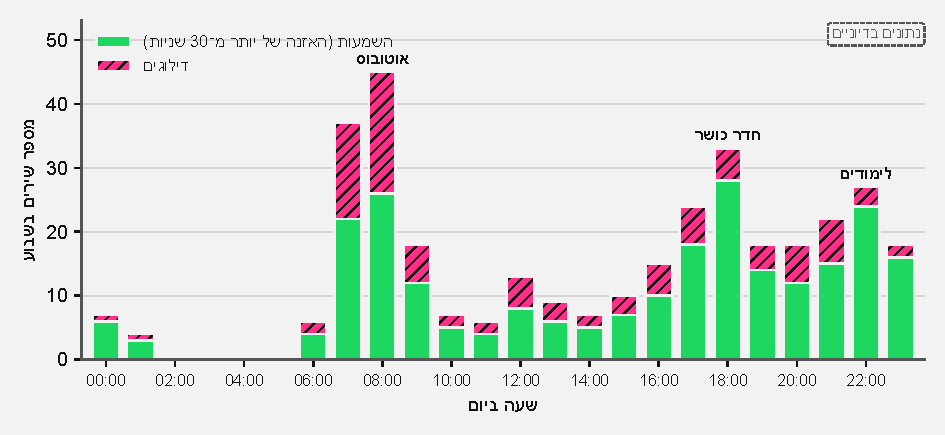
\includegraphics[width=\textwidth]{noa_week.pdf}
\caption{השבוע של נועה \fictional}\label{fig:test}\end{figure}
\begin{table}[htbp]\centering\caption{טבלת בדיקה}\label{tab:test}
\begin{tabularx}{\textwidth}{@{}lXX@{}}\toprule
\textbf{היבט} & \textbf{שיטה א} & \textbf{שיטה ב}\\\midrule
מה משתמשים & הרגלי האזנה של אנשים דומים & תכונות של השיר עצמו\\
שיר חדש? & קשה & אפשרי\\\bottomrule\end{tabularx}\end{table}
\chapter*{מקורות}\begin{english}\printbibliography[heading=none]\end{english}
\end{document}
